\subsection{Forwarding and Routing}

The network layer implements host-to-host communication.
On the sending side, it encapsulates segments into datagrams.
On the receiving side, it delivers segments to the transport layer.
Network layer protocols exist in every host and router.
A router examines the header fields of all IP datagrams passing through it.

The network layer performs forwarding and routing.
Forwarding is the movement of packets from the router input to the appropriate router output.
Routing is the determination of the route taken by packets from their source to their destination.

A routing algorithm determines the end-to-end path through the network.
A forwarding table determines local forwarding within a router.
Before datagrams can flow, the end hosts and intermediate routers establish a virtual connection.

\subsection{Network Service Model}

Channels for transporting datagrams can have different service models.
Services for individual datagrams include guaranteed delivery or guaranteed delivery with less than a specified delay.
Services for a flow of datagrams include ordered delivery, guaranteed minimum bandwidth and restrictions on changes in packet spacing.

The network layer of the Internet provides a single service known as `best effort' service.
Packets are neither guaranteed to be received in order, nor is their eventual delivery guaranteed.
There is also no guarantee on end-to-end delay or minimum bandwidth.

\subsection{Router Input Ports}

The input port of a router consists of a physical layer that receives the data stream from the network and a data link layer that strips the Ethernet header and forwards the remaining IP datagram to the network layer.
Within the network layer, the input port acts as a decentralised switch by performing lookup, forwarding and queueing.
The output port corresponding to the datagram destination is obtained from the local forwarding table.
The goal is to complete input port processing at `line speed' (the input link speed).
If datagrams arrive at a faster rate than the forwarding rate into the switch fabric, queueing occurs.

As there are billions of IP addresses, the forwarding table maps ranges of addresses (aggregate table entries) to output ports.
The corresponding table entry for a given address is the one with the longest matching address prefix.
Packets are transferred from the input buffer to the appropriate output buffer via a switching fabric.
The switching rate is the rate at which packets can be transferred from input to output and is often expressed as a multiple of the input or output line rate.
For \(N\) inputs, a switching rate of no more than \(N\) times the line rate is desirable.

Input port queuing can occur when the fabric is slower than the input ports combined.
Packets may be lost due to buffer overflow.
Head-of-line (HOL) blocking occurs when a datagram at the head of a queue prevents other datagrams from moving forward.

\subsection{Router Switching Fabrics}

The three types of switching fabric are
\begin{enumerate}
  \item memory,
  \item bus, and
  \item crossbar.
\end{enumerate}

\begin{figure}[htp]
  \centering
  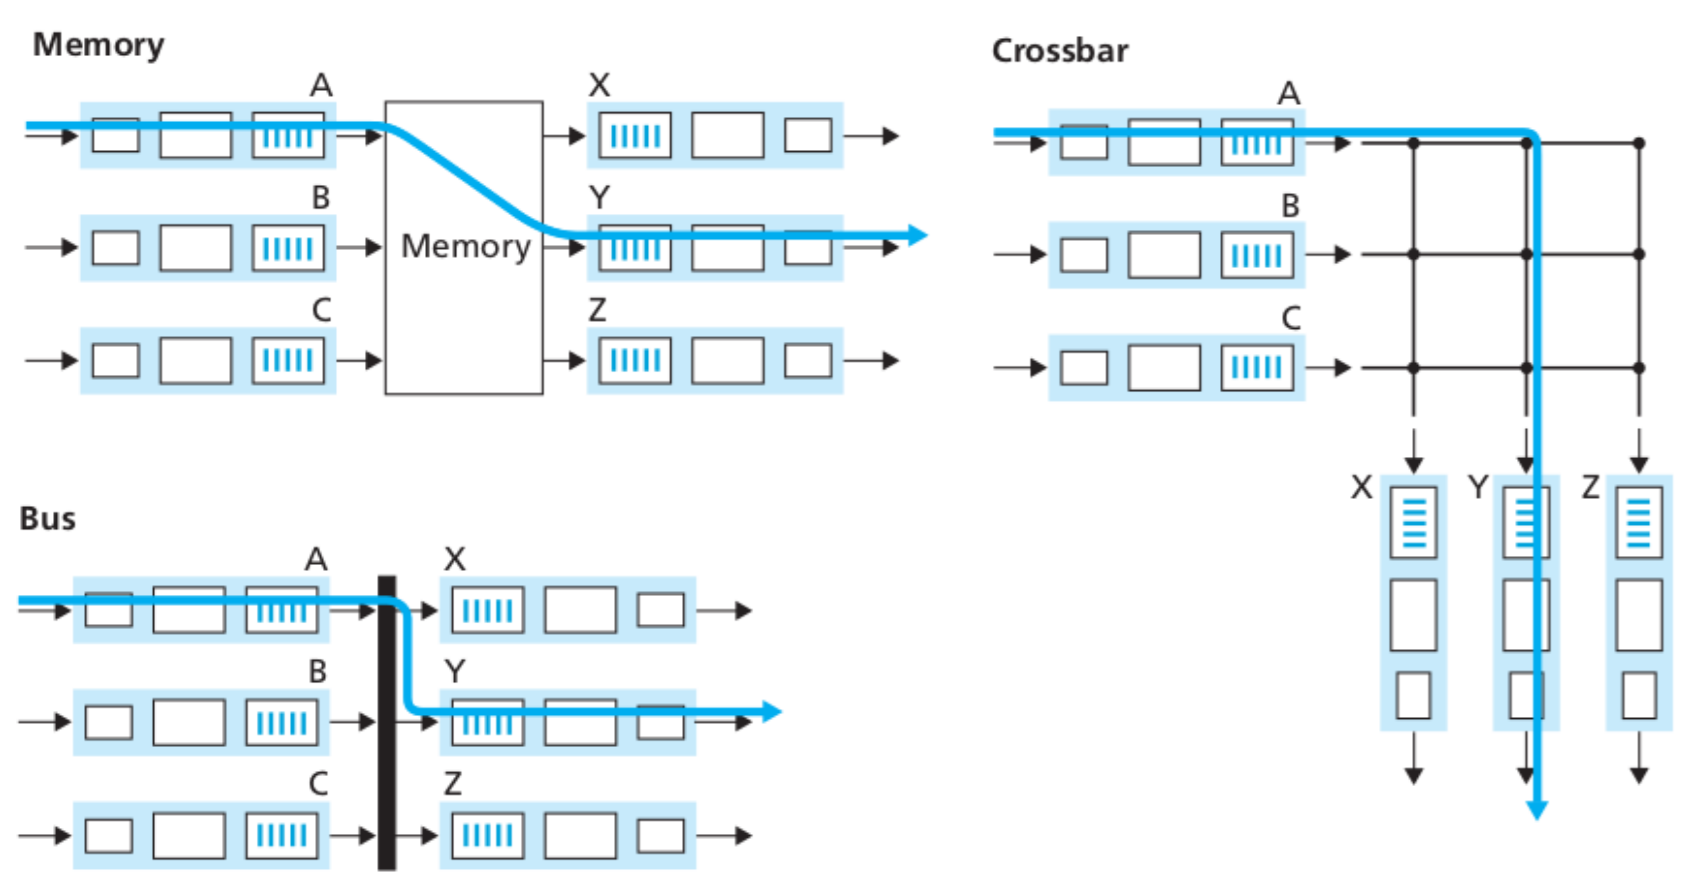
\includegraphics[width=15cm]{unit-19/figures/switching-fabrics.png}
  \caption{The three types of switching fabric.}
\end{figure}

\subsubsection{Memory Switching Fabric}

Memory switching fabrics were used by early routers and traditional computers with switching under direct control of the CPU\@.
The packet is copied to system memory and then to the output.
Speed is limited by memory bandwidth and two bus crossings are required for each datagram.

\subsubsection{Bus Switching Fabric}

Bus switching fabrics are used in routers for access and enterprise networks.
A datagram is transferred from input port memory to output port memory via a shared bus without intervention by the routing processor.
The input port prepends a switch-internal label (header) and transmits the packet onto the bus.
Header matching occurs at the output ports to ensure only the relevant port receives the packet.
Switching speed is limited by bus bandwidth.
This may lead to bus contention.

\subsubsection{Crossbar Switching Fabric}

Crossbar switching fabrics are used in high-bandwidth interconnection network routers.
To overcome bus bandwidth limitations, a crossbar with \(m\) inputs and \(n\) outputs requires \(m + n\) buses.
Crossbars support the forwarding of multiple packets in parallel since a crossbar switch is non-blocking.
Crossbars require an advanced design that allows datagrams to be fragmented into cells of fixed length that are transmitted through multiple switching fabrics.

\subsection{Router Output Ports}

Buffering is required when datagrams arrive from the switching fabric faster than the transmission rate.
A scheduling discipline chooses among the queued datagrams for transmission.
Datagrams (packets) can be lost due to congestion and a lack of buffers.

An old recommendation was that average buffering should be equal to the product of the typical RTT and the link capacity \(C\).
However, an updated recommendation is that the average buffering should be equal to the quotient of that value and the square root of the number \(N\) of TCP flows.

\begin{equation*}
  \frac{\text{RTT} \times C}{\sqrt{N}}
\end{equation*}

\subsection{IP Datagram Fragmentation}

\begin{figure}[htp]
  \centering
  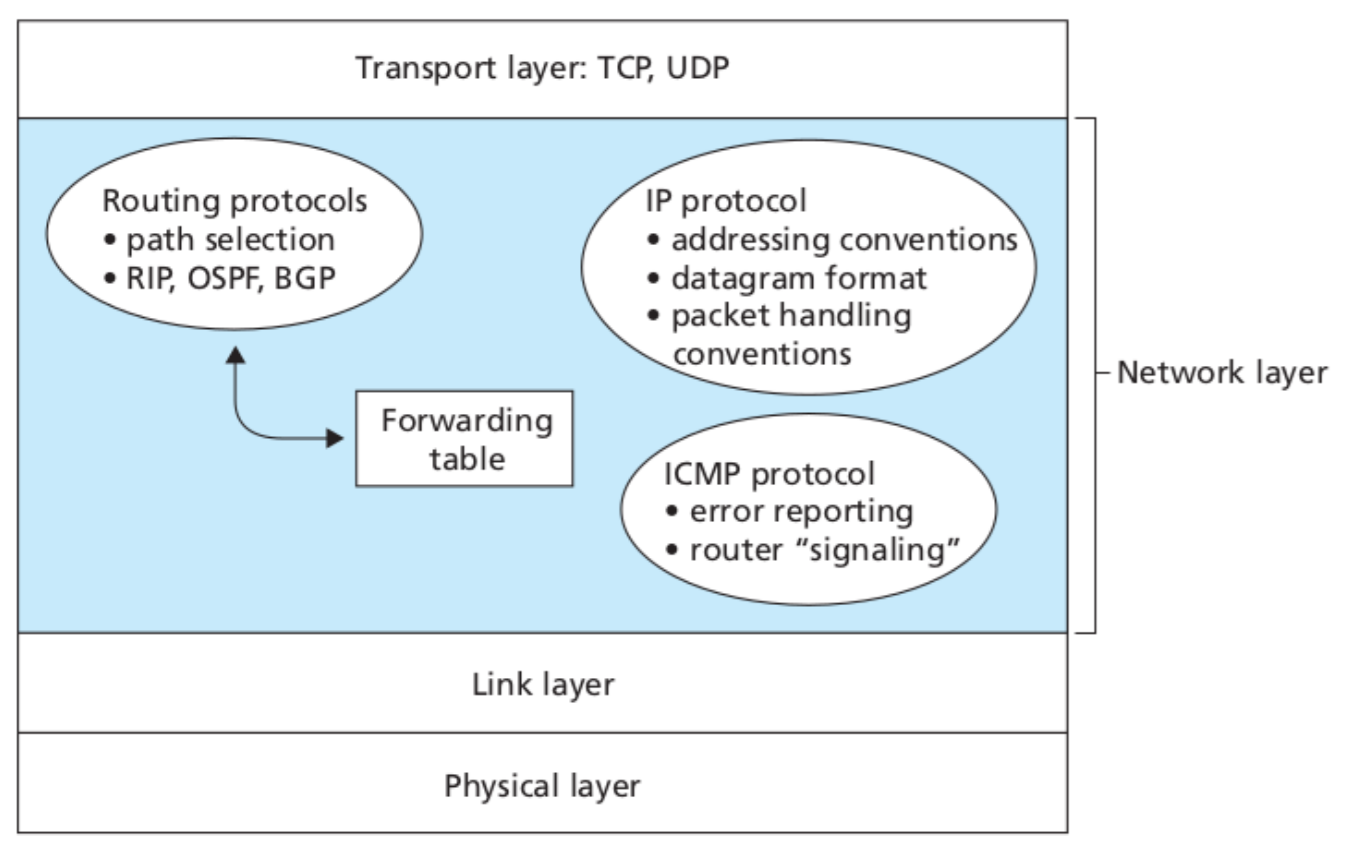
\includegraphics[width=12cm]{unit-19/figures/network-layer.png}
  \caption*{Host and router network layer functions.}
\end{figure}

\begin{figure}[htp]
  \centering
  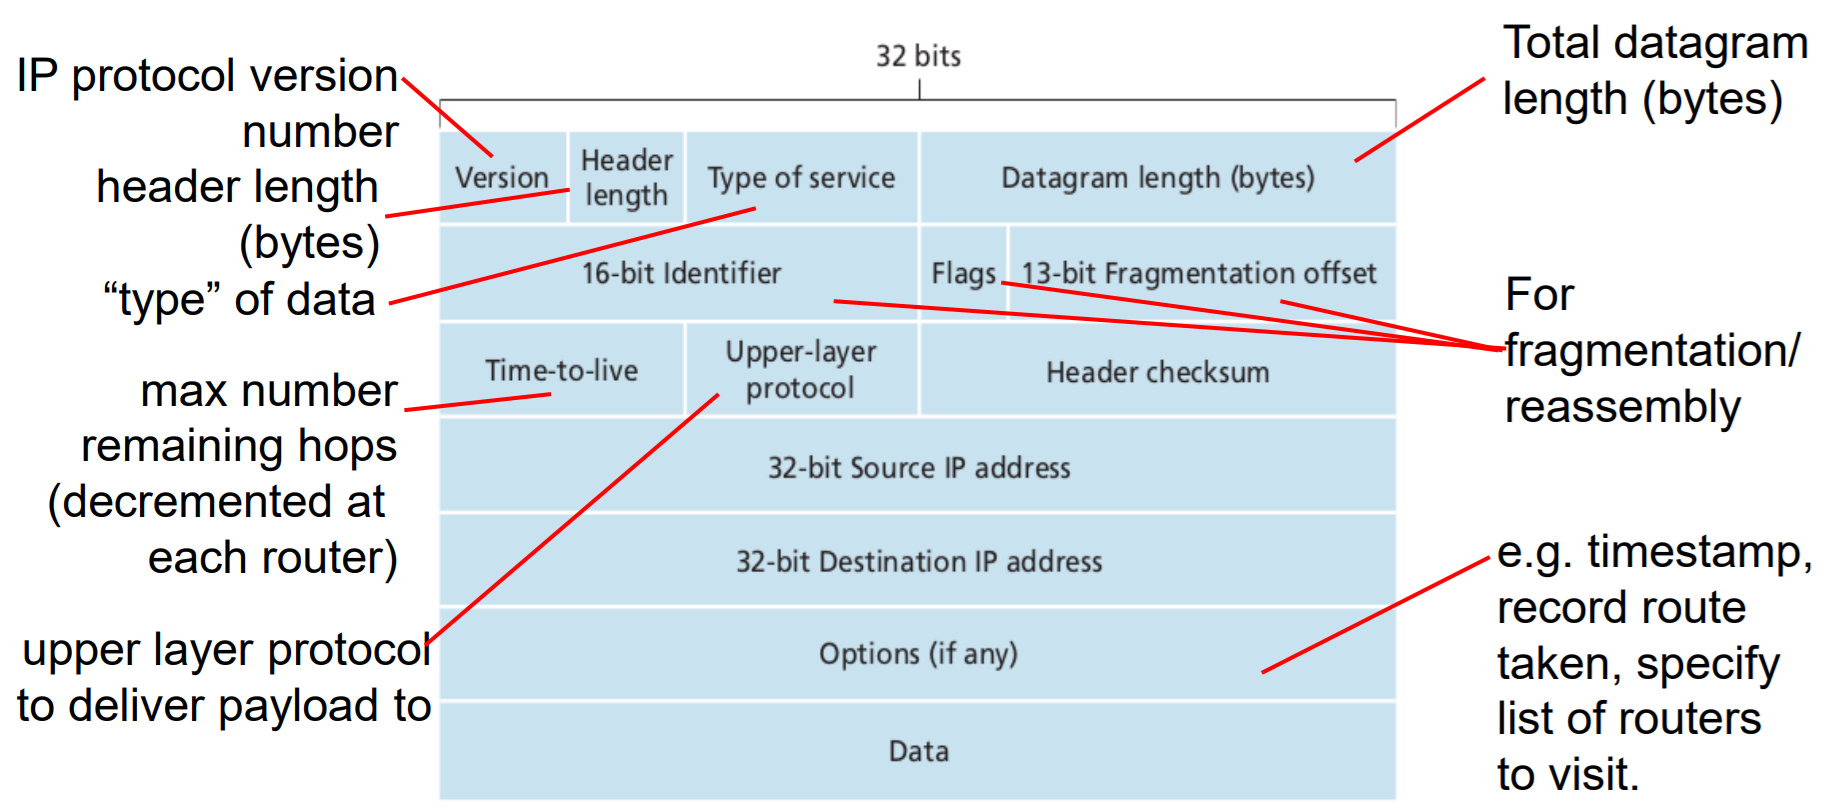
\includegraphics[width=15cm]{unit-19/figures/ip-datagram.png}
  \caption*{The IP datagram format.}
\end{figure}

The header of an IP datagram is \SI{20}{\byte} long.
The total overhead is the sum of \SI{20}{\byte} of IP header, \SI{20}{\byte} of TCP header and the application layer overhead.

Network links have a maximum transmission unit (MTU).
This is the largest possible link-level frame.
Different types of link along a path may have different MTUs.
A large datagram is fragmented within a network and reassembled at its destination.
IP header bits are used to identify and order related fragments.

IP datagrams contain fields for their length, ID, fragmentation flag and offset.
The fragments of an IP datagram have their fragmentation flags set to \num{1}, except for the final fragment, which has a fragmentation flag of \num{0}.
The offset of a fragment is the quotient of the size of the data (the difference between the MTU size and the header size of \SI{20}{\byte}) and the number \num{8}.

\begin{figure}[htp]
  \centering
  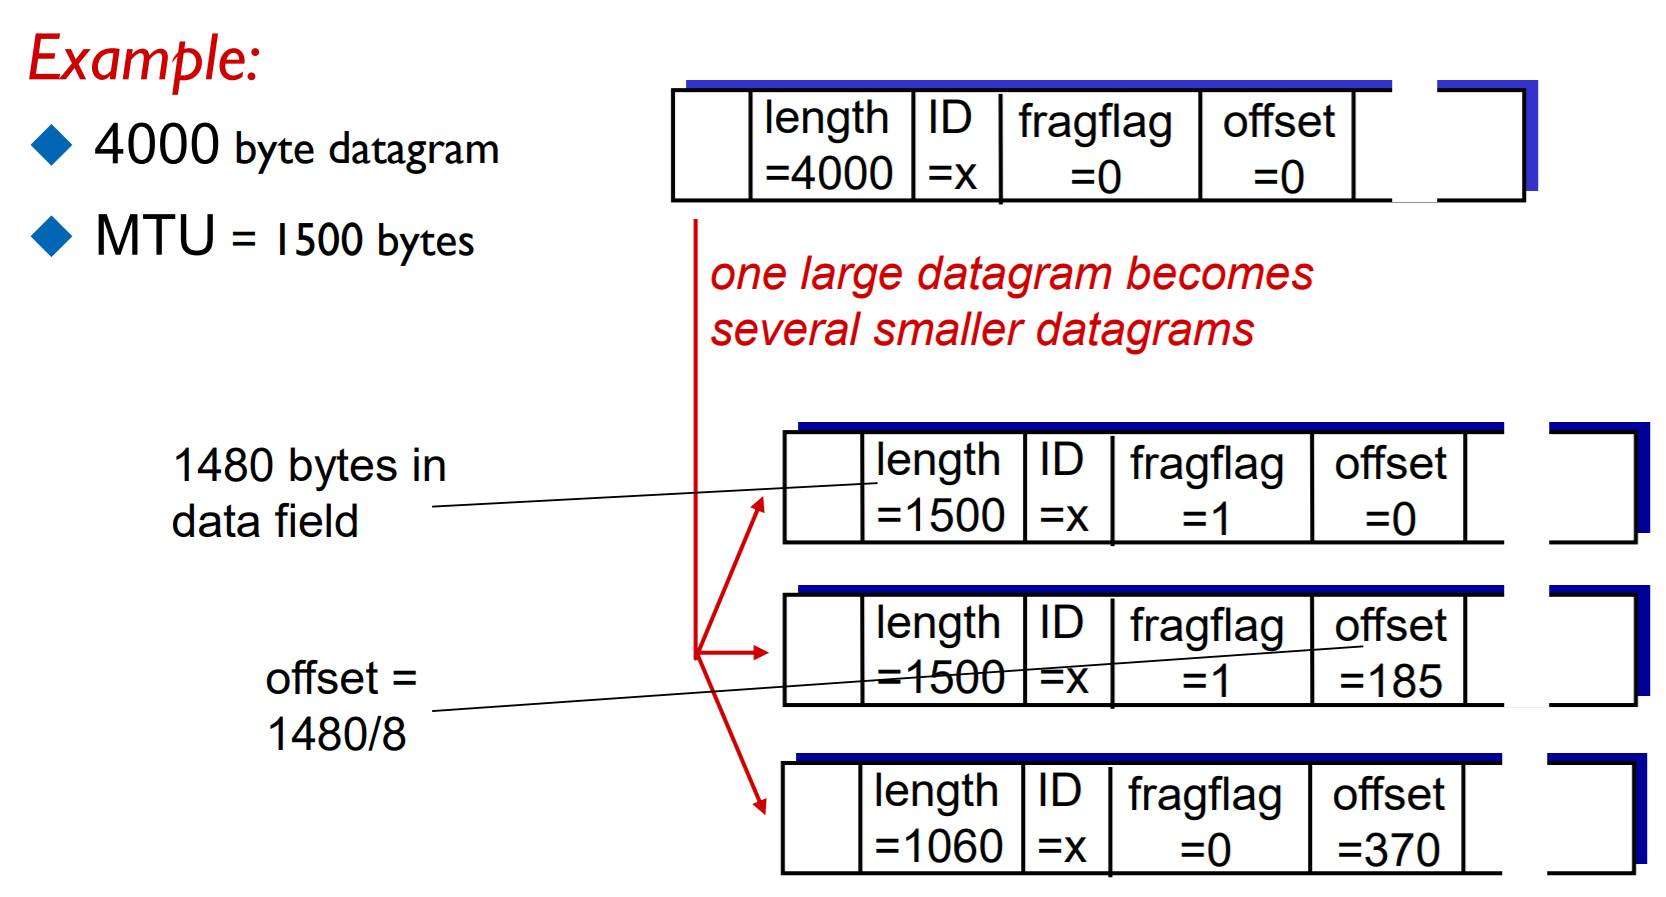
\includegraphics[width=15cm]{unit-19/figures/fragmentation.png}
  \caption*{IP datagram fragmentation.}
\end{figure}

\subsection{IP Addressing}

An IP address is a \SI{32}{\bit} identifier for the host and router interface.
An interface is a connection between the host or router and the physical link.
A router typically has multiple interfaces.
A host can have multiple interfaces for different connection devices, such as Ethernet and wireless.
Each interface has its own IP address.

An IP address consists of a high-order subnet portion and a low-order host portion.
A subnet is a group of interfaces with the same subnet portion of their IP addresses.
Hosts in a subnet can communicate without intervention by the router.

\subsubsection{Classless Interdomain Routing (CIDR)}

Classless Interdomain Routing (CIDR) produces addresses of the format \texttt{a.b.c.d/x}, where \(x\) is the number of bits in the subnet portion of the address.
This allows the subnet portion of the address to be an arbitrary length.

A host can be given a fixed IP address by the system admin, or a dynamic IP address from a DHCP server.

\subsection{Dynamic Host Configuration Protocol (DHCP)}

The goal of the Dynamic Host Configuration Protocol (DHCP) is to allow a host to dynamically obtain its IP address from the network server when it joins.
A host can renew its lease on the address in use, or the address can be reused for a different host that connects.

\begin{itemize}
  \item The host broadcasts a DHCP discover message (optional).
  \item The DHCP server responds with a DHCP offer message (optional).
  \item The host requests an IP address with a DHCP request message.
  \item The DHCP server sends the address in a DHCP acknowledge message.
\end{itemize}

A DHCP server can also return the address of the first-hop router for the client, the name and IP address of the DNS server, and the network mask, which indicates the subnet and host portions of the address.

The subnet portion of an IP address is allocated as a portion of the address space of its ISP\@.
ISPs are allocated address spaces by the Internet Corporation for Assigned Names and Numbers (ICANN), which also manages DNS and assigns domain names.

\subsection{Network Address Translation (NAT)}

Network Address Translation (NAT) ensures that all datagrams leaving a local network have the same single source NAT IP address, but different source port numbers.
This allows a local network to use just one IP address as an interface to the Internet and to change its ISP without having to change the addresses of its local hosts.
Additionally, IP addresses can be changed within the local network without affecting their addresses to the rest of the Internet, and devices within the local network are not explicitly addressable or visible to the outside world.
Only one address is needed from the ISP for all hosts in the network.

A NAT router must replace the source IP address of every outgoing datagram with the NAT IP address and a new port number, store every translation pair in a NAT translation table, and replace the NAT IP address and port number of every incoming datagram with the corresponding source IP address and port number.

NAT uses a \SI{16}{\bit} port number to allow many simultaneous connections with a single IP address.
NAT is controversial since a router should only process up to the network layer.
This violation of the end-to-end agreement must be taken into account by application designers.
The address shortage could instead be solved by using IPv6 addresses.
